
\section{metabolism.xml}

The metabolism file is strongly inspired by SBML.\@
More precisely, it is a subpart of an SBML file.


\subsection{RBAMetabolism}
\label{sec:rba_metabolism}

The outermost portion of the metabolism file is an instance of class
\rbametabolism, shown in Figure~\ref{fig:metabolism_doc}.

\begin{figure}
  \centering
  \includegraphics[scale=0.8]{figures/metabolism_doc}
  \caption{XML structure of metabolism document.}
\label{fig:metabolism_doc}
\end{figure}

Currently, \rbametabolism{} has no simple attributes.
It includes exactly one instance of \textbf{ListOf} container classes.
All \textbf{ListOf} classes do not have own attributes,
they are merely used to organize a list of instances from another class.
This organization was inspired by SBML.\@


\subsection{Compartment}
\label{sec:compartment}

The \compartment{} class is used to list existing cell compartments.

\paragraph{The \textit{id} attribute}
The \textbf{id} attribute is a string defining the identifier of a compartment.


\subsection{Species}
\label{sec:species}

The \species{} class is used to define \emph{metabolic} species.

\paragraph{The \textit{id} attribute}
The \textbf{id} attribute is a string defining the identifier of a metabolite.

\paragraph{The \textit{boundaryCondition} attribute}
The \textbf{boundaryCondition} attribute is a boolean.
If the attribute is set to true, the metabolite is considered to be at
a constant concentration.
In other words, it is not affected by reactions.
This is typical for metabolites in the external medium.


\subsection{Reaction}
\label{sec:reaction}

The \reaction{} class is used to define metabolic reactions
(Fig.~\ref{fig:metabolism_reaction}).
Reactants and products are defined using a \textbf{ListOfSpeciesReferences}.

\begin{figure}
  \centering
  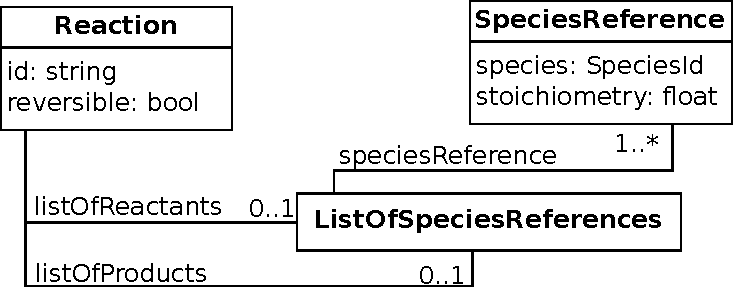
\includegraphics[scale=0.8]{figures/metabolism_reaction}
  \caption{Class storing metabolic reactions.}
\label{fig:metabolism_reaction}
\end{figure}

\paragraph{The \textit{id} attribute}
The \textbf{id} attribute is a string defining the identifier of a reaction.

\paragraph{The \textit{reversible} attribute}
The \textbf{reversible} attribute is a boolean.
If the attribute is set to true, the reaction can occur in both directions.
If the attribute is set to false, only the forward reaction can occur.


\subsection{SpeciesReference}
\label{sec:species_reference}

The \speciesreference{} class is used to refer to a metabolic \species{}
and associate with it a stoichiometry (Fig.~\ref{fig:metabolism_reaction}).

\paragraph{The \textit{species} attribute}
The \textbf{species} attribute must match the identifier of a \species{}.

\paragraph{The \textit{stoichiometry} attribute}
The \textbf{stoichiometry} is a positive real number.
It repensents the stoichiometry of a \species{} in a given context
(typically a \reaction).
